\bluepage{Příprava bufferů}

\begin{frame}\frametitle{Buffers}
\scriptsize
\begin{itemize}
\item An buffer is memory block allocated in device memory of GPU.
\item It can contain any data.
\item The most common usecase is for storing vertices and indices.
\item A buffer can be part of Vertex Array (as vertex buffer or element buffer).
\item For general purposes, it can be bound to \textcolor{red}{GL\_SHADER\_STORAGE\_BUFFER}.
\item A buffer can be used for transform feedback.
\item There are also buffer textures.
\end{itemize}

\begin{itemize}
\item Buffer je objekt zastřešující lineární paměť na GPU.
\item Může obsahovat jakákoliv data.
\item Nejčastěji se používá pro uložení vrcholů geometrie (a jejich vlastností) a indexů na vrcholy.
\item Pro obecné použití může být připojen k \textcolor{red}{GL\_SHADER\_STORAGE\_BUFFER}.
\item Lze jej použít pro transform feedback a pro buffer textury.
\end{itemize}
\end{frame}

\begin{frame}
\frametitle{OpenGL 4.6 pipeline}
  \begin{figure}[h]
  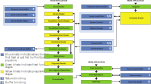
\includegraphics[width=10cm,keepaspectratio]{pics/pipeline/OpenGL460Pipeline}
  \end{figure}
\end{frame}

\definecolor{bg}{rgb}{0.95,0.95,0.95}

\begin{frame}[fragile]
\frametitle{Buffer creation, allocation, data upload}
Buffer creation / Vytvoření bufferu:
\scriptsize
\begin{minted}[bgcolor=bg]{packages/c_cpp.py:CppLexer -x}
float data[]={1,2};//CPU data
GLuint vbo;//buffer handle
glCreateBuffers(1,&vbo);
//allocate buffer and upload data
glNamedBufferData(vbo,sizeof(data),data,GL_DYNAMIC_DRAW);
\end{minted}
Buffer modification / Změna dat v bufferu.
\scriptsize
\begin{minted}[bgcolor=bg]{packages/c_cpp.py:CppLexer -x}
float*ptr;//pointer to data
ptr=(float*)glMapNamedBuffer(vbo,GL_READ_WRITE);//maps the buffer
ptr[0]=0.5;//sets the value
glUnmapNamedBuffer(vbo);//unmap buffer, commits changes
\end{minted}
Different way / Nebo pomoci {\color{blue} glNamedBufferSubData}.
    {\scriptsize
\begin{minted}[bgcolor=bg]{packages/c_cpp.py:CppLexer -x}
glNamedBufferSubData(vbo,
  sizeof(float),//offset
  sizeof(float),//size
  data);//data
    \end{minted}
    }
\end{frame}


